\documentclass[a4paper,12pt]{article}

\textwidth 17cm \textheight 25cm \evensidemargin 0cm
\oddsidemargin 0cm \topmargin -2.5cm
\parindent 0pt
%\parskip \bigskipamount

\usepackage{graphicx}
\usepackage[dutch]{babel}
\usepackage{amssymb,amsthm,amsmath}
\usepackage[utf8]{inputenc}
\usepackage{nopageno}
\usepackage{pdfpages}
\usepackage{enumerate}
\usepackage{caption}
\usepackage{wrapfig}
\usepackage{pgf,tikz}
\usepackage{color}
\usetikzlibrary{arrows}
\usetikzlibrary{patterns}
\usepackage{fancyhdr}
\pagestyle{fancy}
\usepackage[version=3]{mhchem}
\usepackage{multicol}
\usepackage{fix-cm}
\usepackage{setspace}
\usepackage{mhchem}
\usepackage{xhfill}
\usepackage{parskip}
\usepackage{cancel}
\usepackage{mdframed}
\usepackage{url}

\newcommand{\todo}[1]{{\color{red} TODO: #1}}

\newcommand{\degree}{\ensuremath{^\circ}}
\newcommand\rad{\qopname\relax o{\mathrm{rad}}}

\newcommand\ggd{\qopname\relax o{\mathrm{ggd}}}

\def\LRA{\Leftrightarrow}%\mkern40mu}

\newcommand{\zrmbox}{\framebox{\phantom{EXE}}\phantom{X}}
\newcommand{\zrm}[1]{\framebox{#1}}

% environment oefening:
% houdt een teller bij die de oefeningen nummert, probeert ook de oefening op één pagina te houden
\newcounter{noefening}
\setcounter{noefening}{0}
\newenvironment{oefening}
{
  \stepcounter{noefening}
  \pagebreak[0]
  \begin{minipage}{\textwidth}
  \vspace*{0.7cm}{\large\bf Oefening \arabic{noefening}}
}{%
  \end{minipage}
}

\usepackage{calc}

% vraag
\reversemarginpar
\newcounter{punten}
\setcounter{punten}{0}
\newcounter{nvraag}
\setcounter{nvraag}{1}
\newlength{\puntwidth}
\newlength{\boxwidth}
\newcommand{\vraag}[1]{
\settowidth{\puntwidth}{\Large{#1}}
\setlength{\boxwidth}{1.5cm}
\addtolength{\boxwidth}{-\puntwidth}
{\large\bf Vraag \arabic{nvraag} \addtocounter{nvraag}{1}}\vspace*{-0.5cm}
{\marginpar{\color{lightgray}\fbox{\parbox{1.5cm}{\vspace*{1cm}\hspace*{\boxwidth}{\Large{#1}}}}}
\vspace*{0.5cm}}
\addtocounter{punten}{#1}}

% arulefill
\newcommand\arulefill[1][]{
  \ifstrempty{#1}{
    \leavevmode{
      \xrfill[-5pt]{0.3pt}[lightgray]
      \endgraf
    }
    \vspace*{0.2cm}
  }{
    \leavevmode{
      \xrfill[-5pt]{0.3pt}[lightgray]
      \endgraf
      \vspace*{0.2cm}
    }
    \foreach \n in {1,...,#1}{
      \leavevmode{
        \xrfill[-5pt]{0.3pt}[lightgray]
        \endgraf
        \vspace*{0.2cm}
      }
    }
  }
}
% \arules{n}
\newcommand{\arules}[1]{
\mbox{}
\color{lightgray}
%\vspace*{0.05cm}
\foreach \n in {1,...,#1}{
  \vspace*{0.75cm}
  \hrule height 0.3pt\hfill
}\color{black}\vspace*{0.2cm}}

% \arule{x}
\newcommand{\arule}[1]{
\color{lightgray}{\raisebox{-0.1cm}{\rule[-0.05cm]{#1}{0.3pt}}}\color{black}
}

% \abox{y}
\newcommand{\abox}[1]{
\fbox{
\begin{minipage}{\textwidth- 4\fboxsep}
\hspace*{\textwidth}\vspace{#1}
\end{minipage}
}
}

\newcommand{\ruitjes}[1]{
\definecolor{cqcqcq}{rgb}{0.85,0.85,0.85}
\hspace*{-2.5cm}
\begin{tikzpicture}[scale=1.04,line cap=round,line join=round,>=triangle 45,x=1.0cm,y=1.0cm]
\draw [color=cqcqcq, xstep=0.5cm, ystep=0.5cm] (0,-#1) grid (20.5,0);
\end{tikzpicture}
}


\newcommand{\assenstelsel}[5][1]{
\definecolor{cqcqcq}{rgb}{0.65,0.65,0.65}
\begin{tikzpicture}[scale=#1,line cap=round,line join=round,>=triangle 45,x=1.0cm,y=1.0cm]
\draw [color=cqcqcq,dash pattern=on 1pt off 1pt, xstep=1.0cm,ystep=1.0cm] (#2,#4) grid (#3,#5);
\draw[->,color=black] (#2,0) -- (#3,0);
\draw[shift={(1,0)},color=black] (0pt,2pt) -- (0pt,-2pt) node[below] {\footnotesize $1$};
\draw[color=black] (#3.25,0.07) node [anchor=south west] { x};
\draw[->,color=black] (0,#4) -- (0,#5);
\draw[shift={(0,1)},color=black] (2pt,0pt) -- (-2pt,0pt) node[left] {\footnotesize $1$};
\draw[color=black] (0.09,#5.25) node [anchor=west] { y};
\draw[color=black] (0pt,-10pt) node[right] {\footnotesize $0$};
\end{tikzpicture}
}

\newcommand{\getallenas}[3][1]{
\definecolor{cqcqcq}{rgb}{0.65,0.65,0.65}
\begin{tikzpicture}[scale=#1,line cap=round,line join=round,>=triangle 45,x=1.0cm,y=1.0cm]
\draw [color=cqcqcq,dash pattern=on 1pt off 1pt, xstep=1.0cm,ystep=1.0cm] (#2,-0.2) grid (#3,0.2);
\draw[->,color=black] (#2.25,0) -- (#3.5,0);
\draw[shift={(0,0)},color=black] (0pt,2pt) -- (0pt,-2pt) node[below] {\footnotesize $0$};
\draw[shift={(1,0)},color=black] (0pt,2pt) -- (0pt,-2pt) node[below] {\footnotesize $1$};
\draw[color=black] (#3.25,0.07) node [anchor=south west] {$\mathbb{R}$};
\end{tikzpicture}
}

\newcommand{\visgraad}[1]{\begin{tabular}{p{0.5cm}|p{#1}}&\\\hline\\\end{tabular}}

\newcommand{\tekenschema}[2]{\begin{tabular}{p{0.5cm}|p{#1}}&\\\hline\\[#2]\end{tabular}}

% schema van Horner
\newcommand{\schemahorner}{
\begin{tabular}{p{0.5cm}|p{7cm}}
&\\[1.5cm]
\hline\\
\end{tabular}}

% geef tabular iets meer ruimte
\setlength{\tabcolsep}{14pt}
\renewcommand{\arraystretch}{1.5}

\newcommand{\toets}[3]{
\thispagestyle{plain}
\vspace*{-2.5cm}
\begin{tikzpicture}[remember picture, overlay]
    \node [shift={(15.25 cm,-1.6cm)}] {%
        \includegraphics[width=1.8cm]{/home/ppareit/kaa1415/logokaavelgem.png}%
    };%
\end{tikzpicture}

\begin{tabular}{|llc|c|}
\hline
\vspace*{-0.5cm}
&&&\\
Naam & \arule{4cm} & {\Large\bf KA AVELGEM} & \\
\vspace*{-0.75cm}
&&&\\
Klas & \arule{4cm} & {\Large\bf 20...-...-...} & \\
\hline
\vspace*{-0.75cm}
&&&\\
Toets & {\bf #2} & {\large\bf #1} & Beoordeling\\
\vspace*{-0.75cm}
&&&\\
Onderwerp & \multicolumn{2}{l|}{\bf #3} &\\
\hline
\end{tabular}
}

\newcommand{\oefeningen}[1]{

\fancyhead[LE, RO]{\vspace{0.5cm} #1}
%\thispagestyle{plain}

{\bf \Large \centering Oefeningen: #1}

}

\raggedbottom

\newcommand\dom{\qopname\relax o{\mathrm{dom}}}
\newcommand\ber{\qopname\relax o{\mathrm{ber}}}

\newcommand\mC{\qopname\relax o{\mathrm{mC}}}
\newcommand\uC{\qopname\relax o{\mathrm{{\mu}C}}}
\newcommand\C{\qopname\relax o{\mathrm{C}}}

\newcommand\W{\qopname\relax o{\mathrm{W}}}
\newcommand\kW{\qopname\relax o{\mathrm{kW}}}
\newcommand\kWh{\qopname\relax o{\mathrm{kWh}}}


\newcommand\V{\qopname\relax o{\mathrm{V}}}
\newcommand\ohm{\qopname\relax o{\mathrm{\Omega}}}
\newcommand\kohm{\qopname\relax o{\mathrm{k\Omega}}}


\newcommand\N{\qopname\relax o{\mathrm{N}}}

\newcommand\Nperkg{\qopname\relax o{\mathrm{N/kg}}}

\newcommand\Nperm{\qopname\relax o{\mathrm{N/m}}}

\newcommand\gpermol{\qopname\relax o{\mathrm{g/mol}}}


\newcommand\kgperm{\qopname\relax o{\mathrm{kg/m}}}
\newcommand\kgperdm{\qopname\relax o{\mathrm{kg/dm}}}
\newcommand\gpercm{\qopname\relax o{\mathrm{g/cm}}}
\newcommand\gperml{\qopname\relax o{\mathrm{g/ml}}}


\newcommand{\mA}{\;\mbox{mA}}
\newcommand{\A}{\;\mbox{A}}
\newcommand{\MA}{\;\mbox{MA}}

\newcommand{\us}{\;\mu\mbox{s}}
\newcommand\s{\qopname\relax o{\mathrm{s}}}

\newcommand\h{\qopname\relax o{\mathrm{h}}}

\newcommand{\mpers}{\;\mbox{m/s}}
\newcommand{\kmperh}{\;\mbox{km/h}}
\newcommand{\kmpermin}{\;\mbox{km/min}}
\newcommand{\kmpers}{\;\mbox{km/s}}

\newcommand{\mph}{\;\mbox{mph}}

\newcommand{\Hz}{\;\mbox{Hz}}

\newcommand\Gm{\qopname\relax o{\mathrm{Gm}}}
\newcommand\Mm{\qopname\relax o{\mathrm{Mm}}}
\newcommand\km{\qopname\relax o{\mathrm{km}}}
\newcommand\hm{\qopname\relax o{\mathrm{hm}}}
\newcommand\dam{\qopname\relax o{\mathrm{dam}}}
\newcommand\m{\qopname\relax o{\mathrm{m}}}
\newcommand\dm{\qopname\relax o{\mathrm{dm}}}
\newcommand\cm{\qopname\relax o{\mathrm{cm}}}
\newcommand\mm{\qopname\relax o{\mathrm{mm}}}
\newcommand\um{\qopname\relax o{\mathrm{{\mu}m}}}
\newcommand\nm{\qopname\relax o{\mathrm{nm}}}


\newcommand\Gg{\qopname\relax o{\mathrm{Gg}}}
\newcommand\Mg{\qopname\relax o{\mathrm{Mg}}}
\newcommand\kg{\qopname\relax o{\mathrm{kg}}}
\newcommand\hg{\qopname\relax o{\mathrm{hg}}}
\renewcommand\dag{\qopname\relax o{\mathrm{dag}}}
\newcommand\g{\qopname\relax o{\mathrm{g}}}
\newcommand\dg{\qopname\relax o{\mathrm{dg}}}
\newcommand\cg{\qopname\relax o{\mathrm{cg}}}
\newcommand\mg{\qopname\relax o{\mathrm{mg}}}
\newcommand\ug{\qopname\relax o{\mathrm{{\mu}g}}}
\renewcommand\ng{\qopname\relax o{\mathrm{ng}}}

\newcommand\ton{\qopname\relax o{\mathrm{ton}}}

\newcommand\Gl{\qopname\relax o{\mathrm{Gl}}}
\newcommand\Ml{\qopname\relax o{\mathrm{Ml}}}
\newcommand\kl{\qopname\relax o{\mathrm{kl}}}
\newcommand\hl{\qopname\relax o{\mathrm{hl}}}
\newcommand\dal{\qopname\relax o{\mathrm{dal}}}
\renewcommand\l{\qopname\relax o{\mathrm{l}}}
\newcommand\dl{\qopname\relax o{\mathrm{dl}}}
\newcommand\cl{\qopname\relax o{\mathrm{cl}}}
\newcommand\ml{\qopname\relax o{\mathrm{ml}}}
\newcommand\ul{\qopname\relax o{\mathrm{{\mu}l}}}
\newcommand\nl{\qopname\relax o{\mathrm{nl}}}

\newcommand\MJ{\qopname\relax o{\mathrm{MJ}}}
\newcommand\kJ{\qopname\relax o{\mathrm{kJ}}}
\newcommand\J{\qopname\relax o{\mathrm{J}}}

\newcommand\T{\qopname\relax o{\mathrm{T}}}
\newcommand\uT{\qopname\relax o{\mathrm{{\mu}T}}}

\newcommand\grC{\qopname\relax o{\mathrm{{\degree}C}}}

\newcommand\K{\qopname\relax o{\mathrm{K}}}
\newcommand\calperK{\qopname\relax o{\mathrm{cal/K}}}

\newcommand\hPa{\qopname\relax o{\mathrm{hPa}}}
\newcommand\Pa{\qopname\relax o{\mathrm{Pa}}}

\newcommand\dB{\qopname\relax o{\mathrm{dB}}}

\newcommand{\EE}[1]{\cdot 10^{#1}}

\onehalfspacing

%\singlespacing
%\onehalfspacing
%\doublespacing

%\setlength{\headsep}{0cm}

\newenvironment{exlist}[1] %
{ \begin{multicols}{#1}
  \begin{enumerate}[(a)]
    \setlength{\itemsep}{0.8em} }
{ \end{enumerate}
  \end{multicols} }




\begin{document}

\thispagestyle{empty}
\begin{center}
  \begin{mdframed}
  \centering
  \fontsize{40}{50}\selectfont Goniometrische functies
  \end{mdframed}
  \vfill
  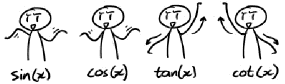
\includegraphics[width=0.7\textwidth]{gon-dance-moves}
  \vfill
\end{center}
\subsection*{Doelstelling}
Je \hfill  {\scriptsize(LP 2005-069, LI 1.4)}
\begin{itemize}
  \item kan de grootte van een hoek uitdrukken in radialen
  \item radialen omzetten in graden en omgekeerd
  \item kan van de functie $f(x)=\sin x$ (met behulp van de grafiek): de tabel, het domein, het bereik, enkele bijzondere waarden, de periodiciteit, het stijgen/dalen en extrema bepalen
  \item kan de grafiek opbouwen van de functie $f(x) = a \sin(bx+c)+d$ en kunnen op deze grafiek de betekenis van $a$, $b$, $c$ en $d$ interpreteren
\end{itemize}

\pagestyle{empty}
\mbox{}
\newpage
\clearpage
\thispagestyle{empty}
%\mbox{}
{\singlespacing \tableofcontents}
\newpage
\clearpage
\pagenumbering{arabic} 

\pagestyle{fancy}
\lhead{}
\rhead{Goniometrische functies}

\onehalfspacing


\section{Hoekeenheden}
Op onze rekenmachine vinden we in \zrm{MODE} 3 soorten hoekeenheden:\\

\textbf{RAD} = radialen

\textbf{DEG} = zestigdelige graden

\textbf{GRA} = honderddelige graden

\subsection{De zestigdelige graad}
Een zestigdelige graad is het 90ste deel van een rechte hoek.\\
\begin{center}
1 rechte hoek = $90\degree$\\
$1\degree = 60'$ (minuten)\\
$1' = 60''$ (seconden)\\
\end{center}
Voor de oorsprong van deze vreemde onderverdeling, in relatie tot ons decimaal talstelsel, moeten we terug naar de Babyloniërs. Voor hen bestond een jaar uit 360 dagen. De kalender was nog lang niet volmaakt, aangezien een totaal van 360 dagen inhield dat om de zoveel jaar extra periodes moesten worden ingelast, de schrikkelmaanden, zodat de kalender gelijk opging met de seizoenen. Uit hun onderzoeken volgde ook de verdeling van de dag in uren, en met behulp van wiskundige berekeningen volgens een zestigtallig stelsel werden de uren opgedeeld in minuten en seconden.
Dit is dezelfde opdeling die wij gebruiken om hoeken te meten!

De zestigdelige graad is nu eenmaal geen zo een handige talstelsel om in te rekenen. Gelukkig hebben wij wiskundigen hier een oplossing voor gevonden. We hebben gewoon nog een nieuwe eenheid ingevoerd, de radiaal!

\pagebreak
\subsection{De radiaal}
De meest natuurlijke hoekeenheid is echter de radiaal. Het woord radiaal is afgeleid van het Latijnse woord ‘radius’, dat straal betekent.

\subsubsection{Definitie}
\begin{minipage}{0.5\textwidth}
De hoekgrootte van een middelpuntshoek waarvan de bijbehorende cirkelboog precies even lang is als de straal van de cirkel, noemen we de {\bf radiaal} ($1 \rad$).
\end{minipage}
\begin{minipage}{0.5\textwidth}
\vspace*{-1cm}
\begin{center}
\definecolor{wqwqwq}{rgb}{0.4,0.4,0.4}
\begin{tikzpicture}[line cap=round,line join=round,>=triangle 45,x=2.0cm,y=2.0cm]
\draw[->,color=black] (-1.5328277784215052,0.) -- (1.6277261422339706,0.);
\foreach \x in {-1.,1.}
\draw[shift={(\x,0)},color=black] (0pt,2pt) -- (0pt,-2pt) node[below] {\footnotesize $\x$};
\draw[->,color=black] (0.,-1.567215720415761) -- (0.,1.3732996361434509);
\foreach \y in {-1.,1.}
\draw[shift={(0,\y)},color=black] (2pt,0pt) -- (-2pt,0pt) node[left] {\footnotesize $\y$};
\draw[color=black] (0pt,-10pt) node[right] {\footnotesize $0$};
\clip(-1.5328277784215052,-1.567215720415761) rectangle (1.6277261422339706,1.3732996361434509);
\draw [shift={(0.,0.)},fill=black,fill opacity=0.1] (0,0) -- (0.:0.30005258740400087) arc (0.:57.29577951308232:0.30005258740400087) -- cycle;
\draw(0.,0.) circle (1);
\draw [shift={(0.,0.)},line width=2.pt]  plot[domain=0.:1.,variable=\t]({1.*1.*cos(\t r)+0.*1.*sin(\t r)},{0.*1.*cos(\t r)+1.*1.*sin(\t r)});
\draw (0.3,0.33) node[anchor=north west] {$1 \rad$};
\draw [line width=1.6pt] (0.,0.)-- (1.,0.);
\draw [line width=1.2pt,dotted] (0.,0.)-- (0.5403023058681398,0.8414709848078965);
\begin{scriptsize}
\draw [fill=wqwqwq] (1.,0.) circle (1.5pt);
\draw [fill=wqwqwq] (0.5403023058681398,0.8414709848078965) circle (1.5pt);
\draw [fill=wqwqwq] (0.,0.) circle (1.5pt);
\end{scriptsize}
\end{tikzpicture}
\end{center}
\end{minipage}

\subsubsection{Verband tussen radialen en zestigdelige graden}

Het getal $\pi$ wordt gedefinieerd als het getal dat we krijgen wanneer we de omtrek van een cirkel delen door de diameter van die cirkel. Dus als we een cirkel met diameter 1 nemen, dan heeft de omtrek lengte $\pi$. Onze éénheidscirkel heeft straal $r=1$, dus de diameter is $2$ en dus de omtrek van de éénheidscirkel is $2\pi$. Hieruit volgt dus dat er voor een volle hoek van $360\degree$ geldt:
\begin{mdframed}
$$360\degree = 2\pi \rad$$
\end{mdframed}


Een rechte hoek meet dus $\frac{\pi}{2}$ en een gestrekte hoek meet dus $\pi \rad$. Omdat de omtrek van de goniometrische cirkel $2\pi$ is, is de maat van de nulhoek niet ondubbelzinnig bepaald. De nulhoek meet zowel $0 \rad$ als $2\pi \rad$. We moeten dus de maatgetallen in radialen slechts op een geheel veelvoud van $2\pi$ na bepalen:

\begin{mdframed}
$$\forall \alpha \in \mathbb{R} : \alpha \rad = (\alpha + k2\pi) \rad (k\in \mathbb{Z})$$
\end{mdframed}

\subsubsection{Graden omzetten in radialen}
We kunnen nu de omzetting berekenen met behulp van het volgende verband:
\begin{alignat*}{2}
     &&360\degree &= 2\pi \rad\\
\LRA &&180\degree &= \pi \rad\\
\LRA &&  1\degree &= \frac{\pi}{180} \rad\\[1em]
\LRA &&  x\degree &= x\cdot\frac{\pi}{180\degree} \rad
\end{alignat*}

\begin{oefening}
Vul de tabel aan met radialen.
\begin{center}
  \begin{tabular}{c|c|c|c|c|c|c|c|c|c}
    $0\degree$ & $30\degree$ & $45\degree$ & $60\degree$ &$90\degree$ &$120\degree$ &$135\degree$ &$150\degree$ &$180\degree$ & $270\degree$ \\
    \hline
   &&&$\frac{1}{3}\pi$&&&&&&\\
  \end{tabular}
\end{center}
\end{oefening}

\subsubsection{Van graden, minuten en seconden naar radialen}

We zetten met het \zrm{ZRM} $309\degree 23' 50''$ om in radialen:

$$309\degree 23' 50''=309\degree 23' 50''\cdot \dfrac{\pi}{180\degree}=5.4\rad$$

\subsubsection{Radialen omzetten in graden}
We kunnen de omzetting berekenen met behulp van het volgende verband:
\begin{alignat*}{2}
     &&2\pi\rad &=360\degree\\
\LRA &&\pi \rad &=180\degree\\
\LRA &&  1 \rad &= \frac{180\degree}{\pi}\\[1em]
\LRA &&  x \rad &= x\cdot\frac{180\degree}{\pi}
\end{alignat*}

\paragraph{Voorbeeld:}
$$5.4 \rad=5.4\cdot\dfrac{180\degree}{\pi}=309\degree 23' 50''$$

\begin{oefening} Zet om in radialen
\begin{multicols}{2}
\begin{enumerate}[(a)]
  \itemsep1em
  \item $75\degree=$\arulefill
  \item $215\degree=$\arulefill
  \item $-75\degree=$\arulefill
  \item $15\degree=$\arulefill
  \item $2.17\degree=$\arulefill
  \item $-35\degree25'47"=$\arulefill
  \item $106\degree20'=$\arulefill
  \item $316\degree2'25"=$\arulefill
\end{enumerate}
\end{multicols}
\end{oefening}

\begin{oefening} Zet om in zestigdelige graden, minuten en seconden
\begin{multicols}{2}
\begin{enumerate}[(a)]
  \item $\pi \rad=$\arulefill
  \item $\dfrac{2\pi}{3} \rad=$\arulefill
  \item $\dfrac{5\pi}{4} \rad=$\arulefill
  \item $\dfrac{-3\pi}{2} \rad=$\arulefill
  \item $\dfrac{\pi}{15} \rad=$\arulefill
  \item $\dfrac{-2\pi}{5} \rad=$\arulefill
  \item $2.86 \rad=$\arulefill
  \item $6 \rad=$\arulefill
  \item $0.456 \rad=$\arulefill
  \item $-0.75 \rad=$\arulefill 
\end{enumerate}
\end{multicols}
\end{oefening}

\subsubsection{Opmerking}
In het vervolg zullen we de eenheid '$\rad$' niet meer vermelden. Wanneer we bv. spreken over een hoek  $\dfrac{2\pi}{3}$, bedoelen we dus steeds  $\dfrac{2\pi}{3} \rad$. Vanaf nu stappen we ook af van de zestigdelige graden en zullen we alles meten in radialen.

\newpage
\section{De goniometrische functies}
\subsection{De sinusfunctie}
\subsubsection{Tabel}
Vul onderstaande tabel aan. De hoek $x$ is uitgedrukt in radialen. Rond af op 2 decimalen.

\begin{adjustwidth}{-2.5cm}{-2.5cm}
\begin{center}
  \begin{tabular}{c|c|c|c|c|c|c|c|c|c|c|c|c}
    $x$ & -1 & 0 & 1 &  $\frac{\pi}{2}$ & 2 & 3 & $\pi$ & 4 & $\frac{3\pi}{2}$ & 5 & 6 & $2\pi$\\
    \hline
   $\sin x$ &\hspace*{0.5cm}&\hspace*{0.5cm}&\hspace*{0.5cm}&\hspace*{0.5cm}&\hspace*{0.5cm}&\hspace*{0.5cm}&\hspace*{0.5cm}&\hspace*{0.5cm}&\hspace*{0.5cm}&\hspace*{0.5cm}&\hspace*{0.5cm}&\hspace*{0.5cm}
  \end{tabular}
\end{center}
\end{adjustwidth}

\subsubsection{Grafiek} 
\begin{center}
\definecolor{cqcqcq}{rgb}{0.75,0.75,0.75}
\definecolor{lightgray}{rgb}{0.95,0.95,0.95}
\begin{tikzpicture}[yscale=1.3,line cap=round,line join=round,>=triangle 45,x=1.0cm,y=1.0cm]
\draw [color=cqcqcq,dash pattern=on 1pt off 1pt, xstep=1.0cm,ystep=1.0cm] (-5.21,-1.47) grid (8.61,1.35);
\draw[->,color=black] (-5.21,0) -- (8.61,0);
\foreach \x in {-5,-4,-3,-2,-1,1,2,3,4,5,6,7,8}
\draw[shift={(\x,0)},color=black] (0pt,2pt) -- (0pt,-2pt) node[below] {\footnotesize $\x$};
\draw[->,color=black] (0,-1.47) -- (0,1.35);
\foreach \y in {-1,1}
\draw[shift={(0,\y)},color=black] (2pt,0pt) -- (-2pt,0pt) node[left] {\footnotesize $\y$};
\draw[color=black] (0pt,-10pt) node[right] {\footnotesize $0$};
\clip(-5.21,-1.47) rectangle (8.61,1.35);
\draw[color=lightgray, line width=1.2pt, smooth,samples=100,domain=-5.211247613943133:8.61062736834769] plot(\x,{sin(((\x))*180/pi)});
\end{tikzpicture}
\end{center}

\subsubsection{Kenmerken van de sinusfunctie}
\begin{oefening}
Vul de kenmerken aan van de sinusfunctie.
\begin{enumerate}[(a)]
  \item $\dom \sin=\arule{3cm}$ en $\ber \sin=\arule{3cm}$
%  \item Periode\\ We merken op dat de sinusfunctie zichzelf steeds herhaalt. We zeggen dat de sinusfunctie periodiek is. De periode van de sinusfunctie is de kleinste afstand waarbij de functie zichzelf herhaalt. Duid deze afstand aan op de grafiek. Voor de sinusfunctie is dit $P=$....................
  \item Nulwaarden:
  \arules{3}
  \item Tekenverloop: 
  \begin{center}
    \visgraad{10cm}
  \end{center}
  \item Stijgen\&dalen en extreme waarden:
  \begin{center}
    \visgraad{10cm}
  \end{center}
\end{enumerate}
\end{oefening}

\subsection{De cosinusfunctie}
\subsubsection{Tabel}
Vul onderstaande tabel aan. De hoek $x$ is uitgedrukt in radialen. Rond af op 2 decimalen.

\begin{adjustwidth}{-2.5cm}{-2.5cm}
\begin{center}
  \begin{tabular}{c|c|c|c|c|c|c|c|c|c|c|c|c}
    $x$ & -1 & 0 & 1 &  $\frac{\pi}{2}$ & 2 & 3 & $\pi$ & 4 & $\frac{3\pi}{2}$ & 5 & 6 & $2\pi$\\
    \hline
   $\cos x$ &\hspace*{0.5cm}&\hspace*{0.5cm}&\hspace*{0.5cm}&\hspace*{0.5cm}&\hspace*{0.5cm}&\hspace*{0.5cm}&\hspace*{0.5cm}&\hspace*{0.5cm}&\hspace*{0.5cm}&\hspace*{0.5cm}&\hspace*{0.5cm}&\hspace*{0.5cm}
  \end{tabular}
\end{center}
\end{adjustwidth}

\subsubsection{Grafiek}
\begin{center}
\definecolor{cqcqcq}{rgb}{0.75,0.75,0.75}
\begin{tikzpicture}[yscale=1.3,line cap=round,line join=round,>=triangle 45,x=1.0cm,y=1.0cm]
\draw [color=cqcqcq,dash pattern=on 1pt off 1pt, xstep=1.0cm,ystep=1.0cm] (-5.21,-1.47) grid (8.61,1.35);
\draw[->,color=black] (-5.21,0) -- (8.61,0);
\foreach \x in {-5,-4,-3,-2,-1,1,2,3,4,5,6,7,8}
\draw[shift={(\x,0)},color=black] (0pt,2pt) -- (0pt,-2pt) node[below] {\footnotesize $\x$};
\draw[->,color=black] (0,-1.47) -- (0,1.35);
\foreach \y in {-1,1}
\draw[shift={(0,\y)},color=black] (2pt,0pt) -- (-2pt,0pt) node[left] {\footnotesize $\y$};
\draw[color=black] (0pt,-10pt) node[right] {\footnotesize $0$};
\clip(-5.21,-1.47) rectangle (8.61,1.35);
\draw[line width=1.2pt, smooth,samples=100,domain=-5.211247613943133:8.61062736834769] plot(\x,{cos(((\x))*180/pi)});
\end{tikzpicture}
\end{center}

\begin{oefening}
Vul de kenmerken aan van de cosinusfunctie.
\begin{enumerate}[(a)]
  \item $\dom \sin=\arule{3cm}$ en $\ber \sin=\arule{3cm}$
%  \item Periode\\ We merken op dat de sinusfunctie zichzelf steeds herhaalt. We zeggen dat de sinusfunctie periodiek is. De periode van de sinusfunctie is de kleinste afstand waarbij de functie zichzelf herhaalt. Duid deze afstand aan op de grafiek. Voor de sinusfunctie is dit $P=$....................
  \item Nulwaarden:
  \arules{3}
  \item Tekenverloop: 
  \begin{center}
    \visgraad{10cm}
  \end{center}
  \item Stijgen\&dalen en extreme waarden:
  \begin{center}
    \visgraad{10cm}
  \end{center}
\end{enumerate}
\end{oefening}

\pagebreak
\subsection{Verband tussen sinus- en cosinusfunctie}

De grafiek van $y=\cos x$ kan je bekomen door deze van $y=\sin x$ met $\frac{\pi}{2}$ eenheden naar links te verschuiven evenwijdig met de $x$-as. Inderdaad, vroeger heb je gezien dat voor de anti-complementaire hoek geldt
$$\sin(x+\dfrac{\pi}{2})=\cos x$$

\subsection{Periode van sinus- en cosinusfunctie}

We merken op dat de sinusfunctie zichzelf steeds herhaalt. We zeggen dat de sinusfunctie periodiek is. De periode van de sinusfunctie is de kleinste afstand waarbij de functie zichzelf herhaalt. Voor de sinusfunctie is dit 
$$p=2\pi\;.$$
We merken op dat er voor de sinusfunctie geldt dat
$$ \sin x = \sin (x+k\cdot 2\pi)\qquad k\in\mathbb{Z}\;.$$

Waarom dit zo is, kan je zien in de volgende figuur:\\
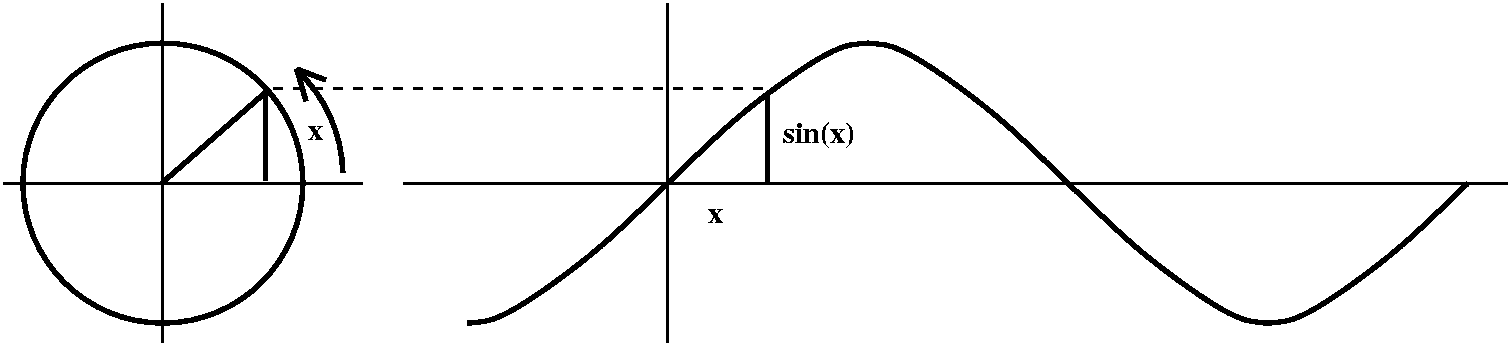
\includegraphics[width=\textwidth]{goniometriccircle_sine}
Breng ook eens een bezoekje aan \verb#http://www.geogebratube.org/student/m8028#, en wijzig daar $\theta$.

\begin{oefening}
Is ook de cosinusfunctie periodiek? Zo ja, bepaal dan de periode:
\arules{3}
\end{oefening}

\paragraph{Definitie}
\begin{mdframed}
Elke reële functie $f$ waarvoor geldt dat er een strikt positief getal $p$ bestaat waarvoor
$$\forall x+k\cdot p \in \mbox{dom} f: f(x)=f(x+k\cdot p)\qquad k\in\mathbb{Z}$$
noemen {\bf periodiek}. De kleinste positieve $p\in\mathbb{R}_0$ noemen we de {\bf periode} van de functie.
\end{mdframed}

\subsection{Amplitude van sinus- en cosinusfunctie}
Bij de sinus- en cosinusfunctie kunnen we de $x$-as als evenwichtsstand nemen. We merken dan op dat de functie steeds uitwijkt van de evenwichtsstand. We zullen de maximale uitwijking vanuit de evenwichtsstand de {\bf amplitude} A noemen.

\begin{oefening}
Bepaal de amplitude
\begin{enumerate}[(a)]
  \item van de sinusfunctie: \arulefill
  \item van de cosinusfunctie: \arulefill
\end{enumerate}
\end{oefening}

De amplitude kan van elke periodieke functie genomen worden die steeds uitwijkt ten opzichte van een evenwichtsstand.

\begin{oefening}
Bepaal voor volgende functie
\begin{center}
\definecolor{cqcqcq}{rgb}{0.7529411764705882,0.7529411764705882,0.7529411764705882}
\begin{tikzpicture}[scale=0.8,line cap=round,line join=round,>=triangle 45,x=1.0cm,y=1.0cm]
\draw [color=cqcqcq,, xstep=1.0cm,ystep=1.0cm] (-5.7606187437084495,-1.794685586926735) grid (5.594801414325579,3.4769983316916453);
\draw[->,color=black] (-5.7606187437084495,0.) -- (5.594801414325579,0.);
\foreach \x in {-5.,-4.,-3.,-2.,-1.,1.,2.,3.,4.,5.}
\draw[shift={(\x,0)},color=black] (0pt,2pt) -- (0pt,-2pt) node[below] {\footnotesize $\x$};
\draw[->,color=black] (0.,-1.794685586926735) -- (0.,3.4769983316916453);
\foreach \y in {-1.,1.,2.,3.}
\draw[shift={(0,\y)},color=black] (2pt,0pt) -- (-2pt,0pt) node[left] {\footnotesize $\y$};
\draw[color=black] (0pt,-10pt) node[right] {\footnotesize $0$};
\clip(-5.7606187437084495,-1.794685586926735) rectangle (5.594801414325579,3.4769983316916453);
\draw [line width=1.6pt] (-6.,3.)-- (-4.,3.);
\draw [line width=1.6pt] (-4.,-1.)-- (-2.,-1.);
\draw [line width=1.6pt] (-2.,3.)-- (0.,3.);
\draw [line width=1.6pt] (0.,-1.)-- (2.,-1.);
\draw [line width=1.6pt] (2.,3.)-- (4.,3.);
\draw [line width=1.6pt] (4.,-1.)-- (6.,-1.);
\end{tikzpicture}
\end{center}
\begin{enumerate}[(a)]
  \itemsep1em
  \item periode $P=\arule{3cm}$
  \item evenwichtsstand $\arule{5cm}$
  \item amplitude $A=\arule{3cm}$
\end{enumerate}
\end{oefening}

\begin{oefening}
Bepaal voor volgende functie
\begin{center}
\definecolor{cqcqcq}{rgb}{0.75,0.75,0.75}
\begin{tikzpicture}[scale=0.8,line cap=round,line join=round,>=triangle 45,x=1.0cm,y=1.0cm]
\draw [color=cqcqcq,dash pattern=on 1pt off 1pt, xstep=1.0cm,ystep=1.0cm] (-3.65,-2.55) grid (6.38,2.25);
\draw[->,color=black] (-3.65,0) -- (6.38,0);
\foreach \x in {-3,-2,-1,1,2,3,4,5,6}
\draw[shift={(\x,0)},color=black] (0pt,2pt) -- (0pt,-2pt) node[below] {\footnotesize $\x$};
\draw[->,color=black] (0,-2.55) -- (0,2.25);
\foreach \y in {-2,-1,1,2}
\draw[shift={(0,\y)},color=black] (2pt,0pt) -- (-2pt,0pt) node[left] {\footnotesize $\y$};
\draw[color=black] (0pt,-10pt) node[right] {\footnotesize $0$};
\clip(-3.65,-2.55) rectangle (6.38,2.25);
\draw[line width=2pt, smooth,samples=100,domain=-3.6545454545454543:6.381818181818182] plot(\x,{1.5*sin((3.1415926535*(\x))*180/pi)});
\end{tikzpicture}
\end{center}
\begin{enumerate}[(a)]
  \itemsep1em
  \item periode $P=\arule{3cm}$
  \item evenwichtsstand $\arule{5cm}$
  \item amplitude $A=\arule{3cm}$
\end{enumerate}
\end{oefening}

\begin{oefening}
Bepaal voor volgende functie
\begin{center}
\definecolor{cqcqcq}{rgb}{0.75,0.75,0.75}
\begin{tikzpicture}[line cap=round,line join=round,>=triangle 45,x=1.0cm,y=1.0cm]
\draw [color=cqcqcq,dash pattern=on 1pt off 1pt, xstep=1.0cm,ystep=1.0cm] (-2.42,-3.36) grid (12.26,2.26);
\draw[->,color=black] (-2.42,0) -- (12.26,0);
\foreach \x in {-2,-1,1,2,3,4,5,6,7,8,9,10,11,12}
\draw[shift={(\x,0)},color=black] (0pt,2pt) -- (0pt,-2pt) node[below] {\footnotesize $\x$};
\draw[->,color=black] (0,-3.36) -- (0,2.26);
\foreach \y in {-3,-2,-1,1,2}
\draw[shift={(0,\y)},color=black] (2pt,0pt) -- (-2pt,0pt) node[left] {\footnotesize $\y$};
\draw[color=black] (0pt,-10pt) node[right] {\footnotesize $0$};
\clip(-2.42,-3.36) rectangle (12.26,2.26);
\draw[line width=1.6pt, smooth,samples=100,domain=-2.4205950413223127:12.259404958677681] plot(\x,{2*sin((3.1415926535*(\x))*180/pi)+sin((2*3.1415926535*(\x)+1)*180/pi)});
\end{tikzpicture}
\end{center}
\begin{enumerate}[(a)]
  \itemsep1em
  \item periode $P=\arule{3cm}$
  \item evenwichtsstand $\arule{5cm}$
  \item amplitude $A=\arule{3cm}$
\end{enumerate}
\end{oefening}

\begin{oefening}
Bepaal voor volgende functie
\begin{center}
\definecolor{cqcqcq}{rgb}{0.75,0.75,0.75}
\begin{tikzpicture}[line cap=round,line join=round,>=triangle 45,x=1.0cm,y=1.0cm]
\draw [color=cqcqcq,dash pattern=on 1pt off 1pt, xstep=1.0cm,ystep=1.0cm] (-5.71,-1.49) grid (8.57,3.21);
\draw[->,color=black] (-5.71,0) -- (8.57,0);
\foreach \x in {-5,-4,-3,-2,-1,1,2,3,4,5,6,7,8}
\draw[shift={(\x,0)},color=black] (0pt,2pt) -- (0pt,-2pt) node[below] {\footnotesize $\x$};
\draw[->,color=black] (0,-1.49) -- (0,3.21);
\foreach \y in {-1,1,2,3}
\draw[shift={(0,\y)},color=black] (2pt,0pt) -- (-2pt,0pt) node[left] {\footnotesize $\y$};
\draw[color=black] (0pt,-10pt) node[right] {\footnotesize $0$};
\clip(-5.71,-1.49) rectangle (8.57,3.21);
\draw[line width=1.6pt, smooth,samples=100,domain=-5.705720690038618:8.570469617334128] plot(\x,{sin((1/2*3.1415926535*(\x))*180/pi)+cos((2*3.1415926535*(\x))*180/pi)+0.85});
\draw (-2.6,1.61) node[anchor=north west] {f};
\end{tikzpicture}
\end{center}
\begin{enumerate}[(a)]
  \itemsep1em
  \item periode $P=\arule{3cm}$
  \item evenwichtsstand $\arule{5cm}$
  \item amplitude $A=\arule{3cm}$
\end{enumerate}
\end{oefening}

\pagebreak
\subsection{De tangensfunctie}
\subsubsection{Tabel}
Vul onderstaande tabel aan. De hoek $x$ is uitgedrukt in radialen. Rond af op 2 decimalen.

\begin{adjustwidth}{-2.5cm}{-2.5cm}
\begin{center}
  \begin{tabular}{c|c|c|c|c|c|c|c|c|c|c}
    x & $\frac{-\pi}{2}$ &-1 & 0 & 1 &  $\frac{\pi}{2}$ & 2 & 3 & $\pi$ & 4 & $\frac{3\pi}{2}$ 
    \\
    \hline
   $\tan x$ &\hspace*{0.5cm}&\hspace*{0.5cm}&\hspace*{0.5cm}&\hspace*{0.5cm}&\hspace*{0.5cm}&\hspace*{0.5cm}&\hspace*{1cm}&\hspace*{0.5cm}&\hspace*{0.5cm}&\hspace*{0.5cm}
  \end{tabular}
\end{center}
\end{adjustwidth}


\subsubsection{Grafiek} 

\begin{center}
\definecolor{uququq}{rgb}{0.25,0.25,0.25}
\begin{tikzpicture}[line cap=round,line join=round,>=triangle 45,x=1.0cm,y=.8cm]
\draw[->,color=black] (-6.72,0) -- (7.5,0);
\foreach \x in {-6,-4,-2,2,4,6}
\draw[shift={(\x,0)},color=black] (0pt,2pt) -- (0pt,-2pt) node[below] {\footnotesize $\x$};
\draw[->,color=black] (0,-3.2) -- (0,3.2);
\foreach \y in {-3,-2,-1,1,2,3}
\draw[shift={(0,\y)},color=black] (2pt,0pt) -- (-2pt,0pt) node[left] {\footnotesize $\y$};
\draw[color=black] (0pt,-10pt) node[right] {\footnotesize $0$};
\clip(-6.72,-3.2) rectangle (7.5,3.2);
\draw[line width=1.2pt, smooth, domain=-7.8:-4.8] plot (\x,{tan(\x*180/pi)});
\draw[line width=1.2pt, smooth, domain=-4.6:-1.6] plot (\x,{tan(\x*180/pi)});
\draw[line width=1.2pt, smooth, domain=-1.5:1.5] plot (\x,{tan(\x*180/pi)});
\draw[line width=1.2pt, smooth, domain=1.6:4.6] plot (\x,{tan(\x*180/pi)});
\draw[line width=1.2pt, smooth, domain=4.8:7.8] plot (\x,{tan(\x*180/pi)});
\draw[line width=1.2pt, smooth, domain=7.9:9] plot (\x,{tan(\x*180/pi)});
\draw (1.15,2) node[anchor=north west] {$y=\tan(x)$};
\end{tikzpicture}
\end{center}

\subsubsection{Kenmerken van de tangensfunctie}
\begin{oefening}
Vul de kenmerken aan van de cosinusfunctie.
\begin{enumerate}[(a)]
  \item $\dom \sin=\arule{3cm}$ en $\ber \sin=\arule{3cm}$
  \item Nulwaarden:
  \arules{3}
  \item Tekenverloop: 
  \begin{center}
    \visgraad{10cm}
  \end{center}
  \item Stijgen\&dalen en extreme waarden:
  \begin{center}
    \visgraad{10cm}
  \end{center}
  \item Periode: $p=\arule{3cm}$
\end{enumerate}
\end{oefening}

\newpage
\section{De algemene sinusfunctie}

\subsection{$\boldsymbol{f(x)=a\cdot\sin x}$ met $\boldsymbol{a\in \mathbb{R}^+_{0}}$}

\subsubsection{Voorbeeld: $\boldsymbol{y=3\cdot\sin x}$}


\begin{adjustwidth}{-2.5cm}{-2.5cm}
\begin{center}
\scriptsize
  \begin{tabular}{c|c|c|c|c|c|c|c|c|c|c|c|c}
    $x$ & -1 & 0 & 1 &  $\frac{\pi}{2}$ & 2 & 3 & $\pi$ & 4 & $\frac{3\pi}{2}$ & 5 & 6 & $2\pi$\\
    \hline
   $\sin x$ &-0.84&0&0.84&1&0.91&0.14&0&-0.76&-1&-0.96&-0.28 &0\\
    \hline
   $3\cdot\sin x$ &-2.52&0&2.52&3&2.73&0.42&0&-2.27&-3&-2.88&-0.84 &0
  \end{tabular}
\end{center}
\end{adjustwidth}

\begin{center}
\definecolor{cqcqcq}{rgb}{0.85,0.85,0.85}
\begin{tikzpicture}[line cap=round,line join=round,>=triangle 45,x=1.0cm,y=1.0cm]
\draw [color=cqcqcq,dash pattern=on 2pt off 2pt, xstep=1.0cm,ystep=1.0cm] (-2.9,-3.4) grid (9.4,3.4);
\draw[->,color=black] (-2.9,0) -- (9.4,0);
\foreach \x in {-2,-1,1,2,3,4,5,6,7,8,9}
\draw[shift={(\x,0)},color=black] (0pt,2pt) -- (0pt,-2pt) node[below] {\footnotesize $\x$};
\draw[->,color=black] (0,-3.4) -- (0,3.4);
\foreach \y in {-3,-2,-1,1,2,3}
\draw[shift={(0,\y)},color=black] (2pt,0pt) -- (-2pt,0pt) node[left] {\footnotesize $\y$};
\draw[color=black] (0pt,-10pt) node[right] {\footnotesize $0$};
\clip(-2.9,-3.4) rectangle (9.4,3.4);
\draw[color=gray, line width=1.2pt, smooth,samples=100,domain=-2.9:9.4] plot(\x,{sin(((\x))*180/pi)});
\draw[line width=1.2pt, smooth,samples=100,domain=-2.9:9.4] plot(\x,{3*sin(((\x))*180/pi)});
\begin{scriptsize}
\draw [color=gray] (1.58,1.46) node[anchor=north west] {$\sin(x)$};
\draw (2.4,2.53) node[anchor=north west] {$3\cdot \sin(x)$};
\end{scriptsize}
\end{tikzpicture}
\end{center}

\subsubsection{Verband tussen $\boldsymbol{y=\sin x}$ en $\boldsymbol{y=3\cdot\sin x}$}
De grafiek van $y=3\cdot\sin x$ bekom je door deze van $y=\sin x$ met een factor 3 verticaal uit te rekken. We spreken van een verschaling evenwijdig met de $y$-as met factor 3.\\
Hierdoor wordt de amplitude A met 3 vermenigvuldigd, terwijl de periode P gelijk blijft:
\begin{center}
  amplitude = A = 3\\
  periode = P = $2\pi$
\end{center}
\subsubsection{Algemeen}
{\bfseries
Voor $\boldsymbol{y=a\cdot\sin x}$ geldt:
  \begin{center}
    Grafiek van $\boldsymbol{y=\sin x}$ verschalen evenwijdig met de $y$-as met factor a:\\
    $\boldsymbol{a>1 \Rightarrow}$ uitrekking\\
    $\boldsymbol{a<1 \Rightarrow}$ inkrimping\\
    Amplitude $\boldsymbol{A = a}$\\
    Periode $\boldsymbol{P = 2\pi}$
  \end{center}
  }

\begin{oefening}
Geef telkens amplitude en periode van volgende functies.
\begin{center}
  \begin{tabular}{c|c|c|c|c}
     & $\sin x$ & $2\cdot\sin x$ &$\frac{1}{2}\cdot\sin x$ & $5\cdot\sin x$\\
    \hline
   Periode P &\arule{2cm} &\arule{2cm}&\arule{2cm}&\arule{2cm}
    \\
    \hline
   Amplitude A &\arule{2cm}&\arule{2cm}&\arule{2cm}&\arule{2cm}
  \end{tabular}
\end{center}
\end{oefening}

\subsection{$\boldsymbol{f(x)=\sin (b\cdot x)}$ met $\boldsymbol{b\in \mathbb{R}^+_{0}}$}
\subsubsection{Voorbeeld: $\boldsymbol{y=\sin (2x)}$}

\begin{adjustwidth}{-2.5cm}{-2.5cm}
\begin{center}
\scriptsize
  \begin{tabular}{c|c|c|c|c|c|c|c|c|c|c|c|c}
    x & -1 & 0 & 1 &  $\frac{\pi}{2}$ & 2 & 3 & $\pi$ & 4 & $\frac{3\pi}{2}$ & 5 & 6 & $2\pi$
    \\
    \hline
   $\sin x$ &-0.84&0&0.84&1&0.91&0.14&0&-0.76&-1&-0.96&-0.28 &0
    \\
    \hline
   $\sin (2x)$ &-0.91 &0 &0.91 &0 &-0.76 &-0.28 &0 &0.99 &0 &-0.54 &-0.54 &0
  \end{tabular}
\end{center}
\end{adjustwidth}

\begin{center}
\definecolor{cqcqcq}{rgb}{0.85,0.85,0.85}
\begin{tikzpicture}[line cap=round,line join=round,>=triangle 45,x=1.0cm,y=1.0cm]
\draw [color=cqcqcq,dash pattern=on 2pt off 2pt, xstep=1.0cm,ystep=1.0cm] (-2.9,-1.9) grid (9.4,1.9);
\draw[->,color=black] (-2.9,0) -- (9.4,0);
\foreach \x in {-2,-1,1,2,3,4,5,6,7,8,9}
\draw[shift={(\x,0)},color=black] (0pt,2pt) -- (0pt,-2pt) node[below] {\footnotesize $\x$};
\draw[->,color=black] (0,-1.9) -- (0,1.9);
\foreach \y in {-1,1}
\draw[shift={(0,\y)},color=black] (2pt,0pt) -- (-2pt,0pt) node[left] {\footnotesize $\y$};
\draw[color=black] (0pt,-10pt) node[right] {\footnotesize $0$};
\clip(-2.9,-1.9) rectangle (9.4,1.9);
\draw[color=gray, line width=1.2pt, smooth,samples=100,domain=-2.9:9.4] plot(\x,{sin(((\x))*180/pi)});
\draw[line width=1.2pt, smooth,samples=100,domain=-2.9:9.4] plot(\x,{sin((2*(\x))*180/pi)});
\begin{scriptsize}
\draw [color=gray] (1.0,1.46) node[anchor=north west] {$\sin(x)$};
\draw (2.80,1.46) node[anchor=north west] {$\sin(2x)$};
\end{scriptsize}
\end{tikzpicture}
\end{center}

\subsubsection{Verband tussen $\boldsymbol{y=\sin x}$ en $\boldsymbol{y=\sin (2x)}$}
De grafiek van $y=\sin (2x)$ bekom je door deze van $y=\sin x$ horizontaal samen te duwen. We spreken van een verschaling  evenwijdig met de $x$-as met factor $\frac{1}{2}$.\\
Hierdoor wordt de periode $P$ door $2$ gedeeld, terwijl de amplitude $A$ gelijk blijft:  
\begin{eqnarray*}
  \mbox{amplitude} &=& A = 1\\
  \mbox{periode} &=& P = \pi
\end{eqnarray*}

\subsubsection{Algemeen}
{\bfseries
Voor $\boldsymbol{y=\sin (bx)}$ geldt:
  \begin{center}
    Grafiek van $\boldsymbol{y=\sin x}$ verschalen evenwijdig met de $x$-as met factor $\boldsymbol{\frac{1}{b}}$:\\
    $\boldsymbol{b>1 \Rightarrow}$ inkrimping\\
    $\boldsymbol{0<b<1 \Rightarrow}$ uitrekking \\
    Amplitude $\boldsymbol{A = 1}$\\
    Periode $\boldsymbol{P = \frac{2\pi}{b}}$
  \end{center}
  }

\begin{oefening}
Geef telkens amplitude en periode van volgende functies.
\begin{center}
  \begin{tabular}{c|c|c|c|c}
     & $\sin x$ & $\sin (3x)$ &$\sin (\frac{1}{2}x)$ & $\sin (5x)$\\
    \hline
    Amplitude A &\hspace*{2cm} &\hspace*{2cm}&\hspace*{2cm}&\hspace*{2cm}
    \\
    \hline
    Periode P &\hspace*{2cm}&\hspace*{2cm}&\hspace*{2cm}&\hspace*{2cm}
  \end{tabular}
\end{center}
\end{oefening}

\subsection{$\boldsymbol{f(x)=\sin (x+c)}$ met $\boldsymbol{c\in \mathbb{R}}$}
\subsubsection{Voorbeeld: $\boldsymbol{y=\sin (x-1)}$}

\begin{adjustwidth}{-2.5cm}{-2.5cm}
\begin{center}
\scriptsize
  \begin{tabular}{c|c|c|c|c|c|c|c|c|c|c|c|c}
    x & -1 & 0 & 1 &  $\frac{\pi}{2}$ & 2 & 3 & $\pi$ & 4 & $\frac{3\pi}{2}$ & 5 & 6 & $2\pi$
    \\
    \hline
   $\sin x$ &-0.84&0&0.84&1&0.91&0.14&0&-0.76&-1&-0.96&-0.28 &0
    \\
    \hline
   $\sin (x-1)$ &-0.91 &-0.84 &0 &0.54 &0.84 &0.91 &0.84 &0.14 &-0.54 &-0.76 &-0.96 &-0.84
  \end{tabular}
\end{center}
\end{adjustwidth}

\begin{center}
\definecolor{cqcqcq}{rgb}{0.85,0.85,0.85}
\begin{tikzpicture}[line cap=round,line join=round,>=triangle 45,x=1.0cm,y=1.0cm]
\draw [color=cqcqcq,dash pattern=on 2pt off 2pt, xstep=1.0cm,ystep=1.0cm] (-2.9,-1.9) grid (9.4,1.9);
\draw[->,color=black] (-2.9,0) -- (9.4,0);
\foreach \x in {-2,-1,1,2,3,4,5,6,7,8,9}
\draw[shift={(\x,0)},color=black] (0pt,2pt) -- (0pt,-2pt) node[below] {\footnotesize $\x$};
\draw[->,color=black] (0,-1.9) -- (0,1.9);
\foreach \y in {-1,1}
\draw[shift={(0,\y)},color=black] (2pt,0pt) -- (-2pt,0pt) node[left] {\footnotesize $\y$};
\draw[color=black] (0pt,-10pt) node[right] {\footnotesize $0$};
\clip(-2.9,-1.9) rectangle (9.4,1.9);
\draw[color=gray, line width=1.2pt, smooth,samples=100,domain=-2.9:9.4] plot(\x,{sin(((\x))*180/pi)});
\draw[line width=1.2pt, smooth,samples=100,domain=-2.9:9.4] plot(\x,{sin(((\x -1))*180/pi)});
\begin{scriptsize}
\draw [color=gray] (1.0,1.46) node[anchor=north west] {$\sin(x)$};
\draw (2.80,1.46) node[anchor=north west] {$\sin(x-1)$};
\end{scriptsize}
\end{tikzpicture}
\end{center}

\subsubsection{Verband tussen $\boldsymbol{y=\sin x}$ en $\boldsymbol{y=\sin (x-1)}$}
De grafiek van $y=\sin (x-1)$ bekom je door deze van $y=\sin x$ horizontaal naar rechts te verschuiven met $1$ eenheid. We spreken van een verschuiving evenwijdig met de $x$-as, bepaald door het koppel $(1, 0)$.\\
Hierdoor blijven de periode $P$ en de amplitude $A$ gelijk.  
\begin{eqnarray*}
  \mbox{amplitude} &=& A = 1\\
  \mbox{periode} &=& P = 2\pi
\end{eqnarray*}

\subsubsection{Algemeen}
{\bfseries
Voor $\boldsymbol{y=\sin (x+c)}$ geldt:
  \begin{center}
    Grafiek van $\boldsymbol{y=\sin x}$ verschuiven evenwijdig met de $x$-as volgens het koppel $\boldsymbol{(-c, 0)}$:\\
    $\boldsymbol{c>0 \Rightarrow}$ c eenheden naar links\\
    $\boldsymbol{c<0 \Rightarrow}$ c eenheden naar rechts \\
    Amplitude $\boldsymbol{A = 1}$\\
    Periode $\boldsymbol{P = 2\pi}$
  \end{center}
  }

\begin{oefening}
Zeg telkens hoe je de grafiek van volgende functies kan bekomen uit deze van $y=\sin x$.
\begin{center}
  \begin{tabular}{c|c|c|c}
    $\sin (x-2)$ & $\sin (x-3)$ & $\sin (x+1)$ & $\sin (x+5)$\\
    \hline
    \hspace*{3cm} &\hspace*{3cm}&\hspace*{3cm}&\hspace*{3cm}
    \\
    &&&
    \\
    &&&
  \end{tabular}
\end{center}
\end{oefening}

\begin{oefening}
Hoe kan je de grafiek van volgende functies bekomen uit deze van de sinusfunctie?
\begin{enumerate}[(a)]
  \item $f(x)=\sin(x-2\pi)$
  \item $f(x)=\sin(x+2\pi)$
  \item $f(x)=\sin(x+4\pi)$
  \item $f(x)=\sin(x+2k\pi)$ met $k\in\mathbb{Z}$
\end{enumerate}
\end{oefening}

\subsection{$\boldsymbol{f(x)=\sin x + d}$ met $\boldsymbol{d\in \mathbb{R}}$} 
\subsubsection{Voorbeeld: $\boldsymbol{y=\sin x-1}$}
\begin{adjustwidth}{-2.5cm}{-2.5cm}
\begin{center}
\scriptsize
  \begin{tabular}{c|c|c|c|c|c|c|c|c|c|c|c|c}
    x & -1 & 0 & 1 &  $\frac{\pi}{2}$ & 2 & 3 & $\pi$ & 4 & $\frac{3\pi}{2}$ & 5 & 6 & $2\pi$
    \\
    \hline
   $\sin x$ &-0.84&0&0.84&1&0.91&0.14&0&-0.76&-1&-0.96&-0.28 &0
    \\
    \hline
   $\sin x-1$ &-1,84& -1& -0.16& 0& -0.09& -0.86& -1& -1,76& -2& -1,96& -1,28 &-1
  \end{tabular}
\end{center}
\end{adjustwidth}

\begin{center}
\definecolor{cqcqcq}{rgb}{0.85,0.85,0.85}
\begin{tikzpicture}[line cap=round,line join=round,>=triangle 45,x=1.0cm,y=1.0cm]
\draw [color=cqcqcq,dash pattern=on 2pt off 2pt, xstep=1.0cm,ystep=1.0cm] (-2.9,-2.9) grid (9.4,1.9);
\draw[->,color=black] (-2.9,0) -- (9.4,0);
\foreach \x in {-2,-1,1,2,3,4,5,6,7,8,9}
\draw[shift={(\x,0)},color=black] (0pt,2pt) -- (0pt,-2pt) node[below] {\footnotesize $\x$};
\draw[->,color=black] (0,-2.9) -- (0,1.9);
\foreach \y in {-1,1}
\draw[shift={(0,\y)},color=black] (2pt,0pt) -- (-2pt,0pt) node[left] {\footnotesize $\y$};
\draw[color=black] (0pt,-10pt) node[right] {\footnotesize $0$};
\clip(-2.9,-2.9) rectangle (9.4,1.9);
\draw[color=gray, line width=1.2pt, smooth,samples=100,domain=-2.9:9.4] plot(\x,{sin(((\x))*180/pi)});
\draw[line width=1.2pt, smooth,samples=100,domain=-2.9:9.4] plot(\x,{sin(((\x))*180/pi)-1});
\begin{scriptsize}
\draw [color=gray] (1.58,1.46) node[anchor=north west] {$\sin(x)$};
\draw (1.0,-0.46) node[anchor=north west] {$\sin(x)-1$};
\end{scriptsize}
\end{tikzpicture}
\end{center}

\subsubsection{Verband tussen $\boldsymbol{y=\sin x}$ en $\boldsymbol{y=\sin x-1}$}
De grafiek van $y=\sin x-1$ bekom je door deze van $y=\sin x$ verticaal naar beneden te verschuiven met 1 eenheid. We spreken van een verschuiving evenwijdig met de $y$-as, bepaald door het koppel $(0, -1)$.\\
Hierdoor blijven de periode $P$ en de amplitude $A$ gelijk.  
\begin{eqnarray*}
  \mbox{amplitude} &=& A = 1\\
  \mbox{periode} &=& P = 2\pi
\end{eqnarray*}

\subsubsection{Algemeen}
{\bfseries
Voor $\boldsymbol{y=\sin x+d}$ geldt:
  \begin{center}
    Grafiek van $\boldsymbol{y=\sin x}$ verschuiven evenwijdig met de $y$-as volgens het koppel $\boldsymbol{(0, d)}$:\\
    $\boldsymbol{d>0 \Rightarrow}$ d eenheden naar boven\\
    $\boldsymbol{d<0 \Rightarrow}$ d eenheden naar beneden \\
    Amplitude $\boldsymbol{A = 1}$\\
    Periode $\boldsymbol{P = 2\pi}$
  \end{center}
  }

\begin{oefening}
Zeg telkens hoe je de grafiek van volgende functies kan bekomen uit deze van $y=\sin x$.
\begin{center}
  \begin{tabular}{c|c|c|c}
    $\sin x-4$ & $\sin x-2$ & $\sin x+3$ & $\sin x+2$\\
    \hline
    \hspace*{3cm} &\hspace*{3cm}&\hspace*{3cm}&\hspace*{3cm}
    \\
    &&&
    \\
    &&&
  \end{tabular}
\end{center}
\end{oefening}

\subsection{De veralgemeende sinusfunctie $\boldsymbol{y=a\cdot \sin[b\cdot (x+c)]+d}$}

\begin{center}
  \fbox{\parbox{\linewidth}{
    {\bfseries
      De functie $\boldsymbol{y=a\cdot \sin[b\cdot (x+c)]+d}$ verloopt sinusoïdaal met\\
      \begin{itemize}
        \item Amplitude $\boldsymbol{A = a}$\\
        \item Periode $\boldsymbol{P=\dfrac{2\pi}{b}}$\\
      \end{itemize}  
      Je kan de grafiek ervan bekomen uit deze van $\boldsymbol{y=\sin x}$ door
      \begin{itemize}
        \item Een verschaling evenwijdig met de $y$-as met factor a\\
          $\boldsymbol{a>1 \Rightarrow}$ uitrekking\\
          $\boldsymbol{0<a<1 \Rightarrow}$ inkrimping\\
        \item Een verschaling evenwijdig met de $x$-as met factor $\boldsymbol{\dfrac{1}{b}}$\\
          $\boldsymbol{b>1 \Rightarrow}$ inkrimping\\
          $\boldsymbol{0<b<1 \Rightarrow}$ uitrekking \\
        \item Een verschuiving evenwijdig met de $x$-as bepaald door het koppel (-c, 0)\\
          $\boldsymbol{c>0 \Rightarrow}$ c eenheden naar links\\
          $\boldsymbol{c<0 \Rightarrow}$ c eenheden naar rechts \\
        \item Een verschuiving evenwijdig met de $y$-as bepaald door het koppel (0, d)\\
          $\boldsymbol{d>0 \Rightarrow}$ d eenheden naar boven\\
          $\boldsymbol{d<0 \Rightarrow}$ d eenheden naar beneden \\
      \end{itemize}}
    }}   
\end{center}
  
\begin{oefening}Bepaal amplitude A en periode P van volgende functies. Zeg telkens in woorden hoe je de grafiek kan bekomen uit deze van $y=\sin x$.\\
\begin{enumerate}[(a)]
  \item $y=\dfrac{1}{2}\cdot\sin [5\cdot(x+\dfrac{\pi}{8})]-3$
  \begin{itemize}
    \itemsep1em
    \item $a=\arule{2cm}\Rightarrow A=\arule{2cm}$
    \item $b=\arule{2cm}\Rightarrow P=\dfrac{2\pi}{b}=\arule{2cm}$
    \item $c=\arule{2cm}$
    \item $d=\arule{2cm}$
    \item Hoe bekom je de grafiek vanuit de sinusfunctie:
    \arules{3}
  \end{itemize}
  \item $\displaystyle y=3\cdot\sin\left(\dfrac{1}{2}x+\pi\right)-4$\\
  \begin{itemize}
    \itemsep1em
    \item $a=\arule{2cm}\Rightarrow A=\arule{2cm}$
    \item $b=\arule{2cm}\Rightarrow P=\dfrac{2\pi}{b}=\arule{2cm}$
    \item $c=\arule{2cm}$
    \item $d=\arule{2cm}$
    \item Hoe bekom je de grafiek vanuit de sinusfunctie:
    \arules{3}
  \end{itemize}
\end{enumerate}
\end{oefening}

\begin{oefening}Geef het voorschrift van de functie die men bekomt door de grafiek van $y=\sin x$
  \begin{enumerate}[(a)]
    \item
    \begin{enumerate}[$\rightarrow$]
      \itemsep0.8em
      \item te verschalen evenwijdig met de $y$-as met factor 2
      \item te verschalen evenwijdig met de $x$-as met factor 3
      \item te verschuiven evenwijdig met de $x$-as met 5 eenheden naar links
      \item te verschuiven evenwijdig met de $y$-as met 4 eenheden naar boven
    \end{enumerate}
    \arules{4}
    \item 
    \begin{enumerate}[$\rightarrow$]
      \itemsep0.8em
      \item te verschalen evenwijdig met de $y$-as met factor $\dfrac{1}{4}$
      \item te verschalen evenwijdig met de $x$-as met factor $\dfrac{1}{5}$
      \item te verschuiven evenwijdig met de $x$-as met 2 eenheden naar rechts
      \item te verschuiven evenwijdig met de $y$-as met 6 eenheden naar beneden
    \end{enumerate}
    \arules{4}
  \end{enumerate}
\end{oefening}

\end{document}
